\clearpage
\subsection{Winkelkorrelation von Vernichtungsphotonen}
Für die Messung der winkelabhängigen Koinzidenzen wurde für verschiedene Winkel mehrere Messungen mit einer Messdauer von jeweils 100s durchgeführt. Es wurde bei Winkeln von $-90^{\circ}$ bis $+90^{\circ}$ gemessen. Hierbei wurde der Plastikszintillator über einem Droharm in die jeweilige Position gebracht, wobei $0^{\circ}$ gerade einem Winkel von $180^{\circ}$ zwischen den beiden Szintillatoren entspricht.\\
An den Einkanaldiskriminatoren des NaJ-Szintillationszählers wurden die Energiefenster so eingestellt, dass möglichst nur Vernichtungsphotonen mit 511 keV registriert werden, d.h. es wurden nur Signale des Peak bei dieser Energie zum Zähler weiter geleitet.\\
Das Delay wurde mit Hilfe des Oszilloskops gewählt. Hierbei wurde die Speicherfunktion genutzt, somit konnte man eine Häufung der Signale feststellen und deren Verzögerung zum anderen festgehaltenen Signal auslesen und justieren.\\
Die Rate zu dein jeweiligen Winkeln berechnet sich wie folgt:
\[ n'(\phi)=\frac{\sum N_i(\phi)}{\sum t_i(\phi)} =: \frac{N_{ges}}{t_{ges}(\phi)} \]
wobei $N_i$ die Anzahl der Ereignisse der $i$-ten Messung und $t_i$ die Messzeit der $i$-ten Messung bei gleichem Winkel $\phi$ ist. Der Fehler der Gesamtrate $n'$ einer Winkeleinstellung $\phi$ lässt sich durch Fehlerfortpflanzung berechnen und erbigt sich durch:
\[ s_{n'}=\frac{1}{\sum t_i} \sqrt{\sum s_{N_i}^2~} = \frac{1}{t} \sqrt{\sum N_i~} = \frac{\sqrt{N}}{t}=\sqrt{\frac{n'}{t}} .\]
Der Fehler auf den Winkel wurde auf $s_{\phi}=0,5^{\circ}$ geschätzt. Die nicht eingekerbten Winkel wurden mit Hilfe einer selbst angefertigten Schablone realisiert. Durch fünf Messungen ohne Probe wurden die durch zufällige Koinzidenzen auftretenden Ereignisse und deren Zählraten bestimmt. Dieser Untergrund wurde von den gemessenen Werten abgezogen, wodurch sich der Fehler auf die vom Untergrund bereinigten Zählraten wie folgt berechnet:
\[ s_n=\sqrt{s_{n'}^2+s_u^2} \]
Auf die aufgetragenen Werte in Abb.\ref{fig:winkelkor} wurde eine Normalverteilung gefittet. 

\begin{figure}[h]
\begin{center}
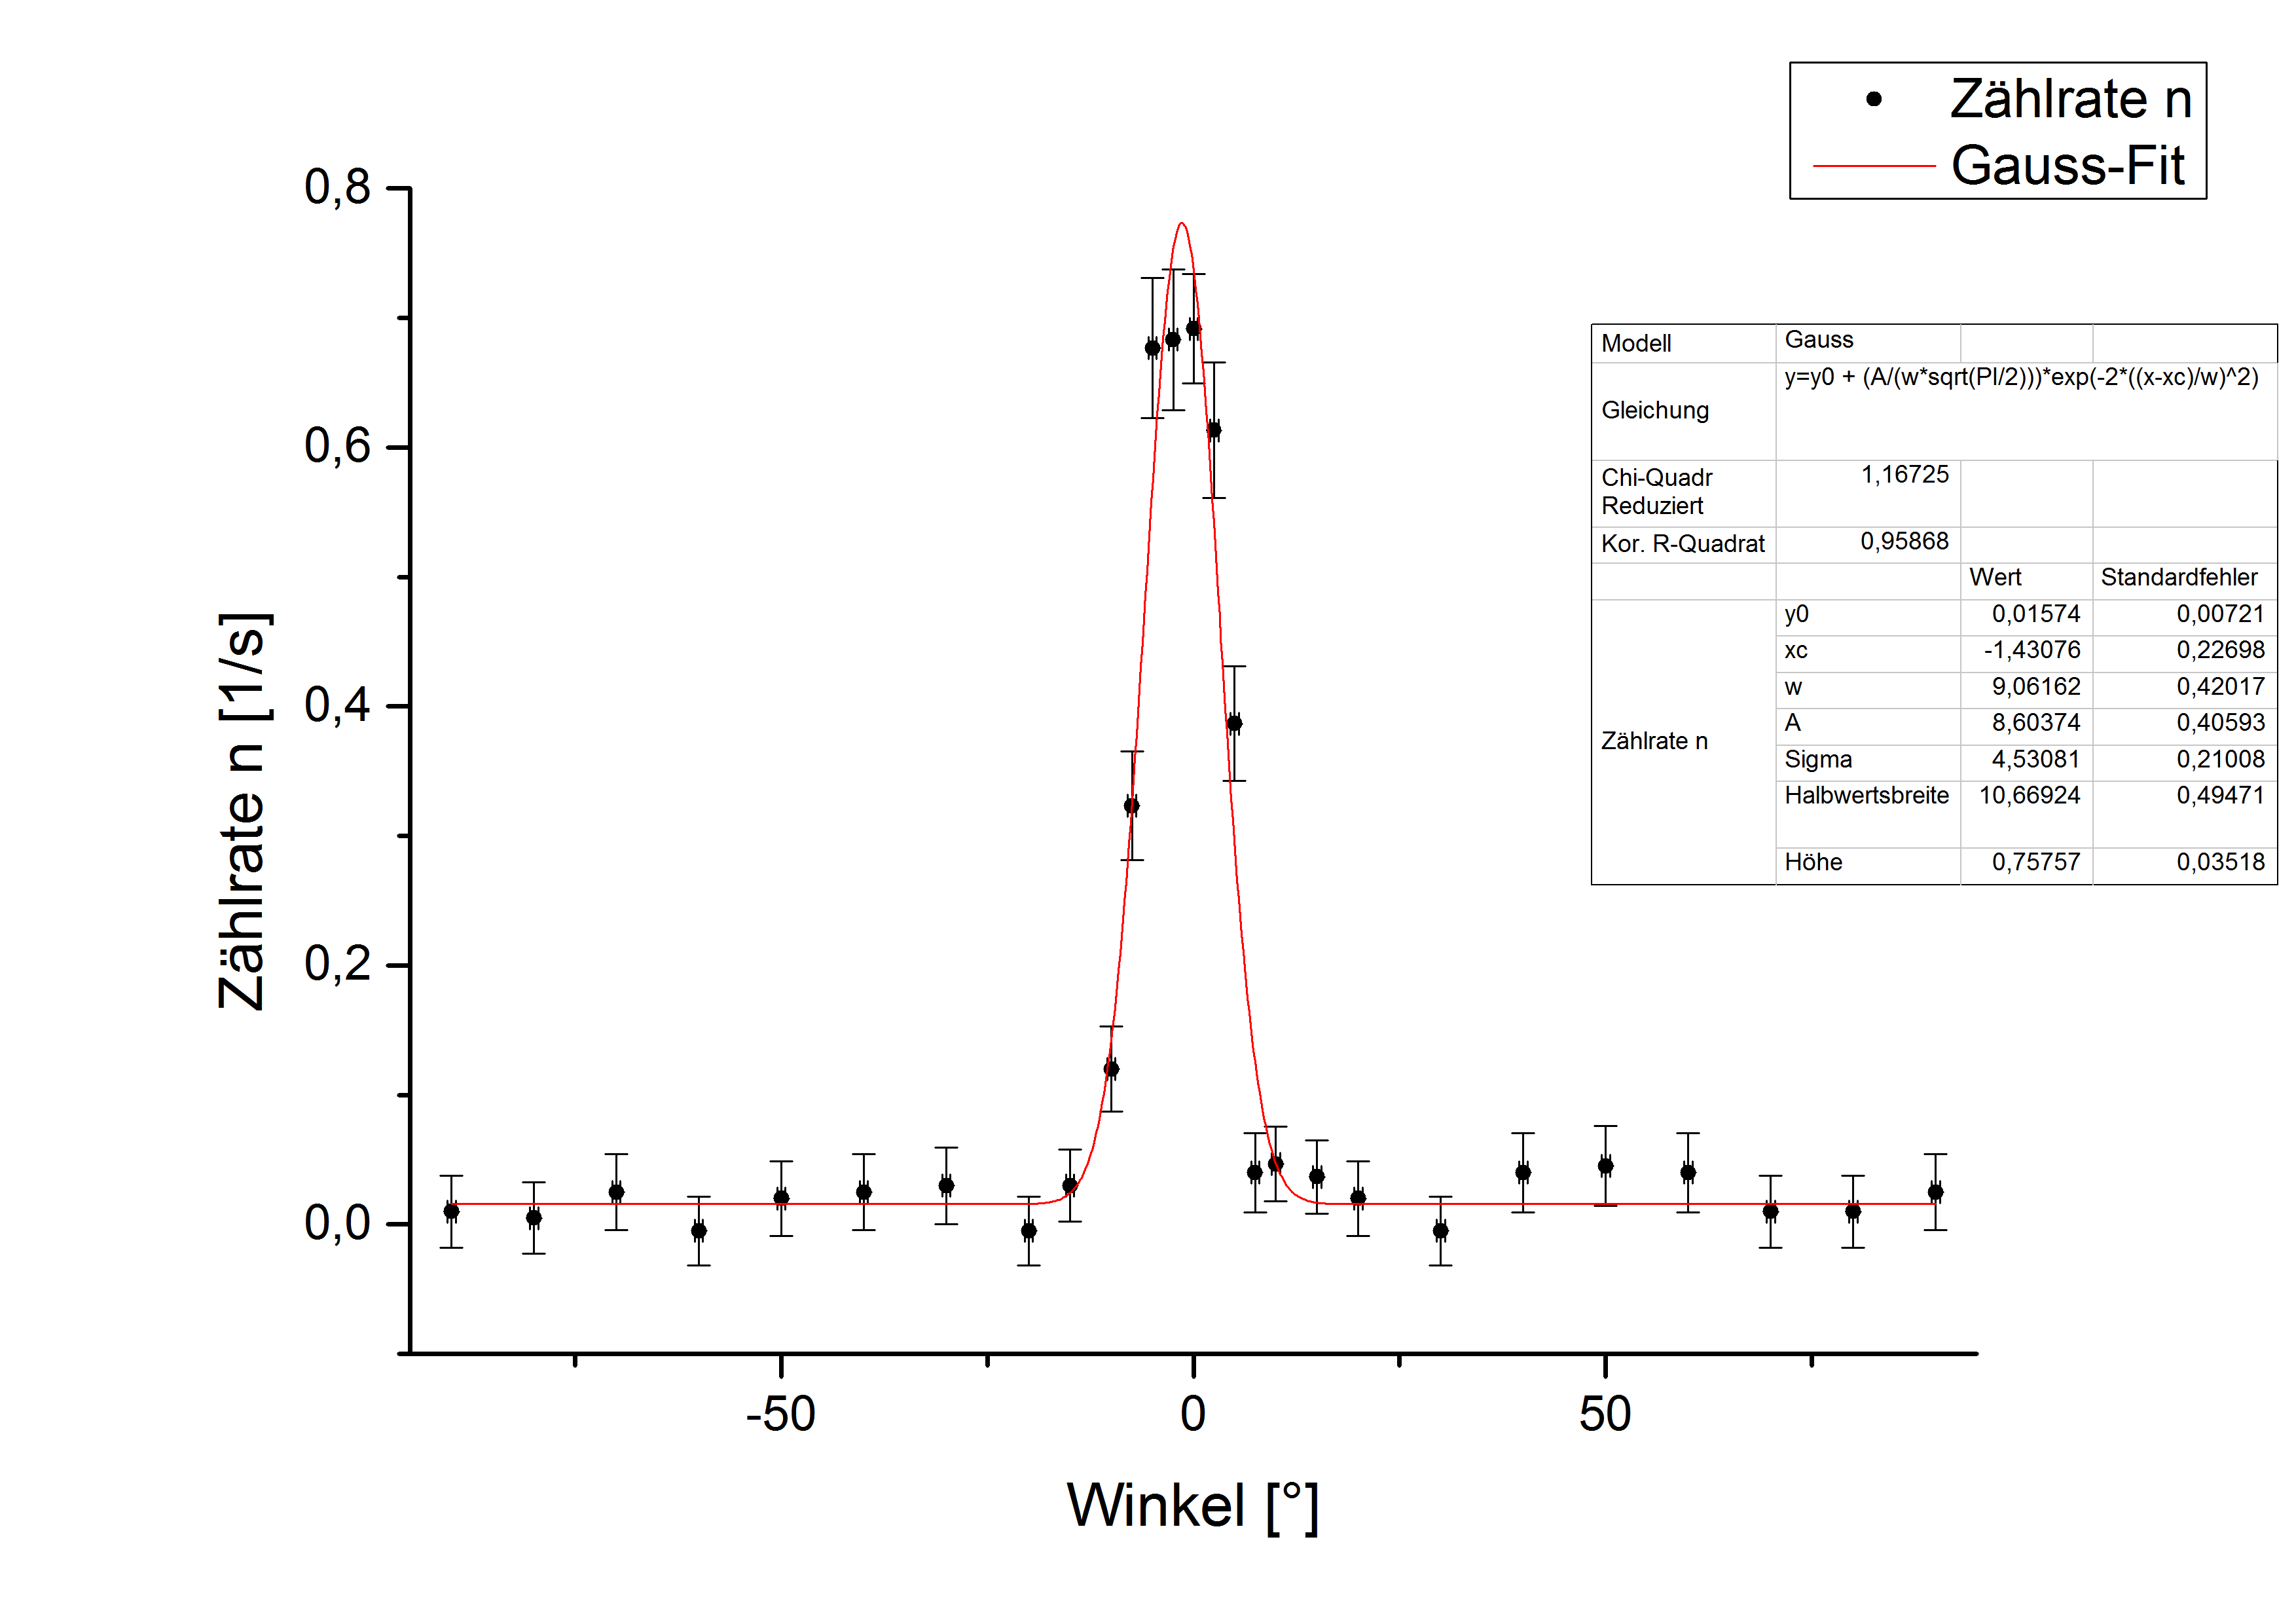
\includegraphics[scale=0.5]{winkelkor}
\caption{Winkelverteilung der Koinzidenzen.}
\label{fig:winkelkor}
\end{center}
\end{figure}

Der von uns gemessene Peak befindet sich bei einem Winkel von $\phi_0 = (-1,4\pm0,2)^{\circ}$ und somit im Rahmen der Messgenauigkeit nicht wie erwartet bei $0^{\circ}$. Diese Abweichung kann dadurch zu Stande kommen, dass die Drehachse nicht exakt zentriert war. Ein weiterer Grund könnte die kurze Messzeit sein, Zerfälle sind zeitlich statistische Ereignisse, für eine qualitativ bessere Aussage benötigt man eine längere Messdauer. In diesem Fall könnte unsere Abweichung eine zufällige Abweichung sein.